\documentclass{bioinfo}
\copyrightyear{2011}
\pubyear{2011}

\bibliographystyle{natbib}
\usepackage{url}  % Formatting web addresses  
 
%%%%%%%%%%%%%%%%%%%%
%% Karro macros   %%
%%%%%%%%%%%%%%%%%%%%
\newcommand{\peace} {{\small PEACE}}
\newcommand{\wcd} {{\small WCD}}
\newcommand{\capthree} {{\small Cap3}}
\newcommand{\easycluster} {{\small EasyCluster}}
\newcommand{\estsim}{{\small ESTSim}}
\newcommand{\metasim} {{\small MetaSim}}
\newcommand{\tgicl} {{\small TGICL}}
\newcommand{\east} {{\small EAST}}
\newcommand{\velvet}{{\small Velvet}}
\newcommand{\mira}{{\small Mira3}}
\newcommand{\pave} {{\small PAVE}}
\newcommand{\peast}{{\small PEACE+EAST}}
 
\usepackage{graphicx}
%\def\includegraphic{}
%\def\includegraphics{}


\begin{document}

\firstpage{1}

\title[EAST transcript assembler]{EAST: \textit{de novo} {\underline E}xpression Fragment {\underline A}ssembly from {\underline S}panning {\underline T}rees}
\author[Zhang \textit{et~al.}]{Yuan Zhang$^1$, Dhananjai M Rao$^1$,
  Mufit Ozden$^1$, Jens Mueller$^2$, Praveen K. Raj Kumar$^4$, Chun
  Liang$^{*1,3}$, John E. Karro$^{*1,4,5}$}

\address{$^1$ Department of Computer Science and Software Engineering, \\
  $^2$ Information Technology Services,
  $^3$ Department of Botany, \\
  $^4$ Department of Microbiology, and
  $^5$ Department of Statistics \\ 
at Miami University, Oxford OHIO, USA
}
\history{Received on XXXXX}

\editor{Associate Editor: XXXXX}

%\title[EAST transcript assembler] 


  %\email{Yuan Zhang - zhangy9@muohio.edu}
  %\and

  %\email{Dhananjai Rao - raodm@muohio.edu}
  %\and

  %\email{Mufit Ozden - ozdenm@muohio.edu}
  %\and

  %\email{Jens Mueller - muellej@muohio.edu}
  %\and

  %\email{Praveen Kumar - rajkump@muohio.edu}
  %\and

  %\email{Chun Liang\correspondingauthor - liangc@muohio.edu}
  %and

  %\email{John E. Karro\correspondingauthor - karroje@muohio.edu}



\maketitle

\textcolor{blue}{
\begin{abstract}
\section{Motivation:} The {\it de novo} assembly of RNA transcript is
computationally challenging problem who importance and difficulty have
both increased with the advent of next generation sequencing
technologies.  The ability to reassemble RNA sequences from a
extremely large dataset of sequence fragment allows not only access to
the transcriptome of unsequenced genomes, but also the exploration and
discovery of novel biological processes.  Hence software tools that
can produce reliable assemblies from large sets of short fragments
from error-prone sequencing technology are in high demand.
\section{Results:} We describe the \east\/ algorithm for the {\it de
  novo} assembly of traditional, short-read, and hybrid
transcript-derived fragments sets, and find that its implementation
results in a tool that appears to be of the most general use (with
respect to multiple sequencing technology platforms) of the tools
examined.  \east\/ consistently outperforms several popular tools on
Sanger sequencing data, out performs or matches competing tools on 454
and hybrid data, and is functional over Illumina data.  In addition,
\east\/ proves to be the most robust tool with respect to sequencing
error.
\section{Availability:} \east\/ can be installed and run through the
\peace\/ GUI, with the implementation and code freely available at
\url{http://www.peace-tools.org}.
\section{Contact:} karrroje@muohio.edu, liangc@muohio.edu
\end{abstract}
}
\section*{Introduction}

\textcolor{blue}{The {\it de novo} assembly of RNA transcripts is an important and
computationally challenging problem, made more difficult by the advent
of Next Generation Sequencing technologies such as 454 and Illumina
[\cite{Nagaraj07}].  Upon completion of transcriptome-sequencing, the
investigator is left with a large set of sequence fragments but no
ordering or transcript association information.  These fragments must
be clustered by transcript and assembled before the sequencing output
can be truly useful.  Access to the relevant organism's genomic
sequence can considerably reduce the complexity of this task, but
using this information is not always an option, or the best option.
{\it de novo} assembly tools assemble the transcript out of the
fragments without using genomic sequence information.  Such tools are
are necessary when working with a genome that is unsequenced
or poorly annotated, but are also useful when in a number of contexts
(for example: when there is limited knowledge of gene splice sites
[\cite{Birol09,Robertson10}]; as an aid in the discovery of novel
biological processes such as transplicing and transcript fusion
[\cite{Mitelman07,Li10b}]; in the annotation of structural variations
not contained within the genome [\cite{Li08}]).}

%\vspace{3mm}

The problem of {\it de novo} transcript assembly has been addressed a
number of times in the literature, with initial approaches
concentrating on the longer reads produced by traditional Sanger
Sequencing techniques, and newer approaches looking at produces of
Next Generation Sequencing (NGS) technologies.  A list of popular
tools addressing these problems include \capthree, \tgicl, \velvet,
and \mira, each excelling within their own context
[\cite{Huang99,Pertea03,Chevreux04,Zerbino08}].  \capthree\/ and
\tgicl\/ use alignment-based strategies that produce high quality
results when applied to the output of Sanger sequencing technologies.
\velvet, based on the modeling of the problem with {\it de bruijn}
graphs, was designed to handle short read sequences.  \mira\/ is a
multi-pass DNA assembler based on an overlap-layout-consensus strategy
that also has an increased ability to assemble {\it hybrid sets}: sets
formed by the mixture of sequencing results from multiple technologies
[\cite{MiraWeb}].

%\vspace{3mm}

\textcolor{blue}{Here we present a novel Minimum Spanning Tree (MST) approach to the
problem of assembling short read, traditional, and hybrid transcript
sequence sets, and show it to be a viable approach through its
implementation in our \east\/ assembly tool.  The tool has been
integrated into the \peace\/ clustering tool set [\cite{Rao10}],
freely available from \url{www.peace-tools.org}.  After a description
of the underlying assembly algorithm, we present a comparison of
\east\/ against \capthree, \tgicl, \velvet, and \mira\/ on multiple
sequencing technology platforms.}

%%%%%%%%%%%%%%%%%%
\section*{Methods}

The algorithm underlying \east\/ is based on three components: minimum
spanning trees (MSTs) [\cite{Prim57}], the $d^2$ sequence distance
measure [\cite{Hide94}], and standard sequence alignment
[\cite{Needleman70,Smith81}].  The objective is to find overlapping
fragments input set and assemble them into contiguous segments
(contigs).  While we would ideally be using sequence alignment to
identify these overlapping ends, the quadratic runtime of alignment
algorithms coupled with the large number of sequences in the input
makes such an approach infeasible.  To avoid excessive alignment
computation, we make use of MSTs to provide a {\it guide} through the
EST set, dictating which pairs are to be aligned.  A modified version
of $d^2$, an alignment-free method for estimating sequence distance,
provides the edge weights for the graph model, allowing us to
construct the MST.

%\vspace{3mm}

\east\/ is an assembly tool, and requires clustering be
done as a pre-processing step, as well as requiring that $d^2$-based
MSTs be provided for each cluster.  Conveniently, the \peace\/
clustering tool [\cite{Rao10}] provides exactly this information.  While
\peace\/ and \east\/ are technically two tools, \east\/ was designed
specifically for \peace\/ output.  For purposes of this paper, it
makes sense to consider them as one.  In the following we briefly
outline the \peace\/ algorithm for clustering (as is relevant to
\east\/), and then discuss the steps taken by \east\/ for assembly of
the \peace\/ clusters.

\subsection*{\peace Clustering}

Given a set of fragments from two or more transcripts, we must first
cluster the fragments by transcript association -- leaving us with a
single cluster of fragments for each transcript.  Details of the
\peace\/ algorithm can be found in {\it Rao et al.} [\cite{Rao10}],
with the general idea as follows: we model the problem as a weighted,
undirected graph, representing each fragment with a node and assigning
edge weights based on a $d^2$ comparison of the incident fragments
(explained in more detail below).  By employing the $u/v$ and $t/v$
filtering heuristics of {\it Hazelhurst et al.} [\cite{Hazelhurst08}],
we can quickly dismiss most of the edges as irrelevant
(i.e. connecting fragments with no overlap), then use Prim's algorithm
to compute an MST [\cite{Prim57}].  Upon completion of the MST we
remove all edges exceeding a specified threshold value, taking each
component of the resulting forest as a cluster.  As a result, \peace\/
passes to \east\/ a set of clusters, an MST for each cluster, and the
orientation of each fragment relative to the cluster.

\subsection*{Overlap Detection}

Given the \peace\/ generated MST for a cluster, the challenge is to
identify and align the ends of overlapping fragments without taking
the significant runtime hit needed to align every pair.  This is
accomplished using two methods: aligning only those sequences adjacent
in the MST, and restricting such alignments to portions identified by
a modified form of the $d^2$ heuristic.

%\vspace{3mm}

A \peace-generated MST represents a single transcript, with each edge
serving as a heuristic indication that the incident sequences overlap;
were there not sufficient sequence similarity to indicate an overlap,
the edge would have initially been assigned a high $d^2$ value and
would have been removed by \peace\/.  To determine exactly how the
nodes overlap, we calculate a modified $d^2$ score as follows.  The
standard calculation of $d^2$, requires looking at every pair of
length $w$ sub-strings (windows) from the two sequences, calculating a
distance between these two windows based on the number of shared words
(6-mers), and taking the score of the lowest-scoring window pairs as
the $d^2$ distance [\cite{Hide94}].  However, when looking for overlap
of fragments $s_1$ and $s_2$, we are looking only for end-overlap.
That is, we wish to determine if the left end of $s_1$ overlaps the
right end of $s_2$, or the reverse (recalling that \peace\/ has
ensured they are on the same strand).  Hence we need only consider the
left-most and right-most windows of $s_1$ against each window of
$s_2$, reducing the number of window comparisons from quadratic to
linear in the size of $s_2$.

%\vspace{3mm}

In Figure~\ref{fig:overlap} we illustrate the use of modified $d^2$,
using it to take two sequences (a), find the window on $s_2$ most
resembling the right-most window of $s1$ (red section of (b)),
extending to the end of $s_2$ (green section of (c)) and performing a
{\it global} alignment on the overlapping portion.  We then compute the
{\it overlap distance} ($1 - s/l$, where $s$ is the alignment score and
$l$ is the length of the overlap segment), a value that is inversely
proportional to the probability that this is a legitimate overlap.

\begin{figure}
\centerline{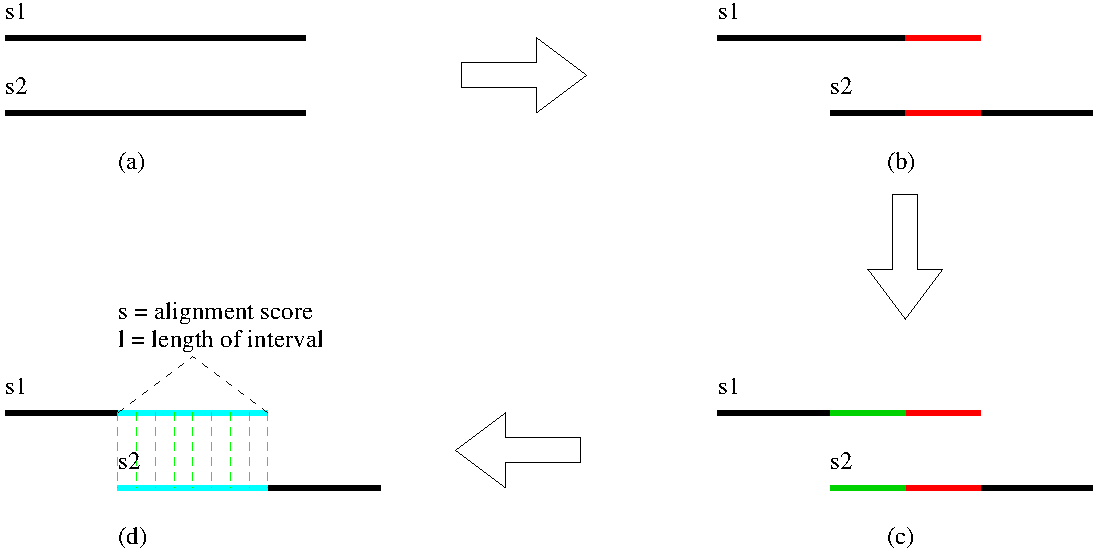
\includegraphics[width=3in]{pics.d/overlap_alignment.pdf}}
\caption{(a) Two sequences potentially overlapping at the ends.  (b)
  The window of $s_2$ pairing with the right-most window of $s_1$ to
  minimize the $d^2$ score.  (c) An extension of the $s_2$ window to
  the end of the sequence, and the corresponding extension on $s_1$.
  (d) A global alignment of the overlapping areas determined from
  (c).}\label{fig:overlap}
\end{figure}


In order to accommodate a range of potential fragment lengths, \peace\/
and \east\/ make use of an {\it adaptive $d^2$} strategy to handle
hybrid data sets.  The $d^2$ measure (and our modification) is
flexible enough to handle a range of sequence sizes, requiring only a
modification of the parameters (i.e. window size and threshold
values).  However, it runs into problems when comparing sequences of
significantly different sizes.  Comparing a 62 base Illumina read
against a 1000 base Sanger read requires the use of parameters
appropriate to the shorter fragment -- which are considerably less
accurate when applied to the longer read.  Our solution is to
partition fragments by sizes (e.g. into groups of small, medium and
large fragments), and compute distances only between segments in the
same or neighboring groups.  By skipping the comparisons between
sequences of significantly different sizes we avoid the pitfalls of
such comparisons, while still implicitly discovering those connections
through transitivity.

\subsection*{Ordering and Reconstruction}

Having defined overlap distance, ordering the fragments is
straight-forward.  We pick an arbitrary node on the cluster's MST and
transverse the tree, using the overlap distance measure to check each
node against its two neighbors.  Those nodes with no identified
left-overlap are checked against nodes further out in the tree, and
any then remaining with no identified left neighbor as designated as a contig
left end.

%\vspace{3mm}

Having identified the distance of each node from its two closest
overlapping sequences, we now construct a {\it directed} graph, with
each edge pointing from a sequence to a right neighbor and weighted
with the overlap distance.  Using this graph we calculate a new
minimum spanning tree, then starting from the root of the tree
(necessarily a left-end of the contig) we transverse the tree and
assign the first base of each sequence a position relative to its
parent.  Such an assignment gives us an implicit ordering of the
fragments.  By scanning through them in order and aligning each to
the next with the Smith-Waterman alignment we end up with a multiple
alignment of the fragments that allows us to derive a consensus
sequence.  During this process quality score information can also be
incorporated, reducing the score contribution of a specific base-pair
if the involved bases are of low quality.  A straightforward extension
would also allow the predictions of single nucleotide polymorphism by
identifying those positions whose covering ESTs vary more in content
than could reasonably be accounted for by the base-call rate.

\noindent{\bf Implementation:} \east\/ has been integrated into the
\peace\/ clustering package [\cite{Rao10}] and is available for
download from the \peace\/ website (\url{www.peace-tools.org}).
Users can run the GUI provided by that site, and through it
install both the \peace\/ cluster engine and \east\/ assembly engine
on a local machine or remote server.
Initial EST data must be in fasta format for fastaq format, though the tool can print
out the final assembly in fasta, ACE, SAM and BAM formats [\cite{Li09}].

 
%%%%%%%%%%%%%%%%%%%%%%%%%%%%
%% Results and Discussion %%
%%
\section*{Results}

In assessing result quality, we must view the \peace\/ clustering tool
[\cite{Rao10}] and \east\/ as a combined process.  Given a unordered
set of fragments representing multiple transcripts, \peace\/ is given
the task of (ideally) producing a minimum spanning tree for each transcript,
with edges representing a subset of the overlap information.  \east\/
then assembles each cluster into one or more contigs.  As most tools
integrate the clustering and assembly process, for purposes of
comparison we must consider our tools as a single tool \peast, and
assess the quality of these results.

%\vspace{3mm}

In order to assess the quality of (\peace\/ +) \east\/ results, we
compared against four prominent assembly tools: \capthree, \tgicl,
\mira, and \velvet\/ [\cite{Huang99,Pertea03,Chevreux04,Zerbino08}].
The tools were tested on data from three sequencing technologies
(Sanger, 454 and Illumina).  Test data was produced using a set of
zebra fish transcripts \cite{Hazelhurst08} and deriving simulated
simulated fragment sets using bot the \estsim\/ and \metasim\/ tools
[\cite{Hazelhurst03,Richter08}].

\subsection*{Measuring Quality}
Our primary measure of quality was the {\bf normalized a-score}, based
on the {\it assembly score} (a-score) used in {\it Liang et al.}
[\cite{Liang00}].  After reconstruction a (portion) of a transcript,
the a-score of that contig is defined as $2c - 5m - 15i$ where $c$ is
the length of the reconstructed contig, $m$ is the number of
miss-called bases, and $i$ is the number of indels.  A ``perfect''
score would be equal to twice the sequence length.  Our normalized
a-score normalizes of the length $t$ of the transcript being
reconstructed, resulting in a formula of:
$$\frac{2s - 5m - 15i}{2t}.$$
Thus a perfect score would be equal to 1.  This normalization allows
for the comparison of assembly quality between sequences of different
lengths. Further, using this score we can more accurately quantify the
quality of a partial reconstruction: if we are able to reconstruct
only a portion of a fragment, the normalized a-score will take full
consideration of the quality of the reconstruction, but then bound the
score by the relative size of the reconstruction.  (For example, were
a tool only able to reconstruct a contig covering one fourth of a
transcript -- but able to reconstruct that portion perfectly -- the
resulting contig's normalized a-score would be $0.25$.)  In addition
we look at: the number of contigs produced by a tool normalized by the
number of transcripts (a value equal to 1 in a perfect
reconstruction); the number of singleton ESTs in the solution
(i.e. ESTs unassigned to any contig and thus, most cases, effectively
thrown away); and the runtime of the tool.

\subsection*{Tool Comparisons}
Using simulated fragment sets allows us to compare assemblies to a
known correct solution and control parameters in their model
(e.g. base-call error rate) to test the effect of variation.  All sets
were generated from a collection of 100 zebra fish transcripts
obtained from {\it Hazelhurst et al.}  [\cite{Hazelhurst08}].  For
Sanger sequences we used the \estsim\/ tool to generated simulated
fragment sets, taking its default model of EST generation when not
otherwise specified [\cite{Hazelhurst03}].  For 454 and Illumina sets
we used the \metasim\/ tool, again using taking their default model to
simulate the errors associated with those technologies
[\cite{Richter08}].  Each tool models potential sequencing mistakes
such as base-call errors, insertion and deletions, using parameters
tailored to the target the technologies; see those publications for
details.

%\vspace{3mm}

\noindent {\bf Sanger Sequencing:} We first compare the assembly
quality of the tools on a Sanger Sequencing model, using \east,
\capthree, and \tgicl\/ (tools designed to work with Sanger
sequences).  The quality of any assembly will be directly affected by
the {\it coverage} of the input: the average number of ESTs that cover
a based.  Thus we investigate the a-score as a function of error rate
at different coverage levels.  For each parameter combination we
applied each tool to 30 independent sets, derived from 15 randomly
chosen members of our zebra fish transcript set, reporting the average
normalized a-score.  In Figure~\ref{sangerAscore} we look at
normalized a-score as a function of error rate, fixing coverage at 50,
30 and 10 and varying base read error rate from 0\% to 6\% for each of
the three tools designed for Sanger Sequencing.  While all three tools
perform well when applied to error free (i.e. impossible) sequencing
technology, we find \east\/ to be considerably more robust to
base-call errors than the other tools.  Taking the mid-range coverage
value of 30 as an example, at a 1\% error rate we see \east,
\capthree, and \tgicl\/ all achieving an essentially perfect
normalized a-score.  At a 3\% error rate \east\/ maintains its almost
perfect normalized a-score, showing a 2\% improvement over \tgicl\/
and a 21\% improvement over \capthree.  At a 4\% error rate \east\/
still maintains its near-perfect score (showing a 54\% and 85\%
improvement over \capthree\/ and \tgicl\/ respectively).  Even at a
6\% error rate \east\/ is still achieving a normalized a-score of 0.95
(a 110\% improvement over the next closest tool, \tgicl\/), meaning
that at most 5\% of the bases were left out of their contigs or were
incorrectly reconstructed.


\begin{figure*}[htb]
\centerline{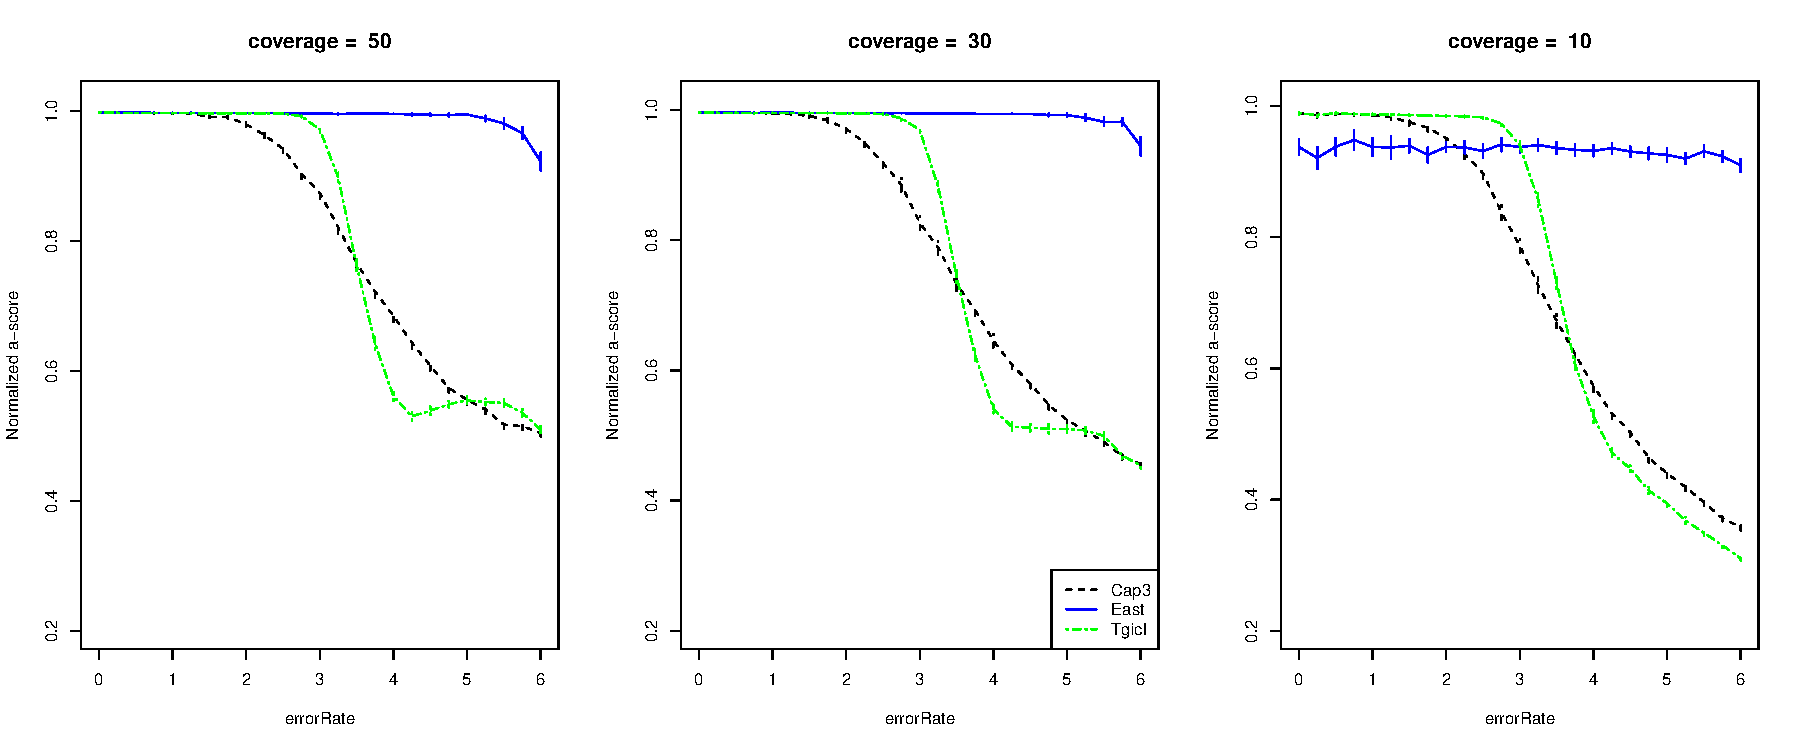
\includegraphics[width=6in]{pics.d/ascore_sanger_norm.pdf}}
\caption{Average normalized a-score as a function of base error rate for
  simulated Sanger sequencing.  \east=blue, \capthree=Black,
  \tgicl=green. COMMENT: Need to change figure heading to Normalized a-score.}
\label{sangerAscore}
\end{figure*}

In Figures~\ref{contigsSanger} is a plot of the average number of
contigs per gene sequence as a function of error rate (top row), the
number of singletons is shown on the bottom row.  For the first we
observe that all tools have comparable results for lower error rates,
but only \east\/ is able to maintain the low score with increasing
error rates -- generating a perfect score in almost every case.  In
minimizing the number of singletons, we find that \east\/ does a
better job than \capthree\/ for error rates larger than $2\%$, while
\tgicl\/ does a better job that \east\/ for error rates larger than
$4\%$ to $5\%$.

\begin{figure*}[htb]
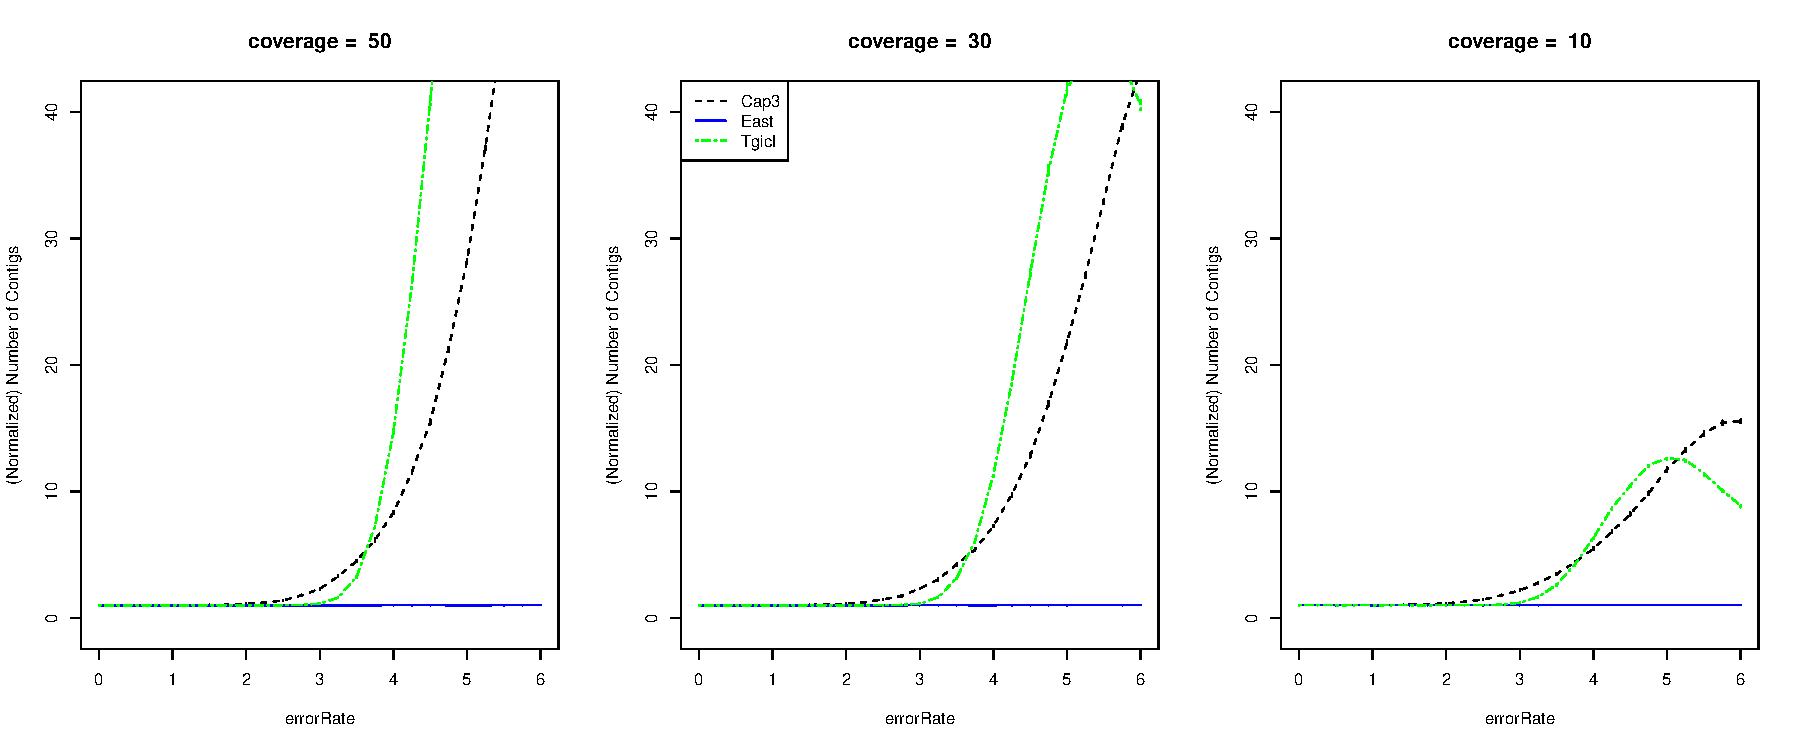
\includegraphics[width=6in]{pics.d/numContigs_sanger.pdf}
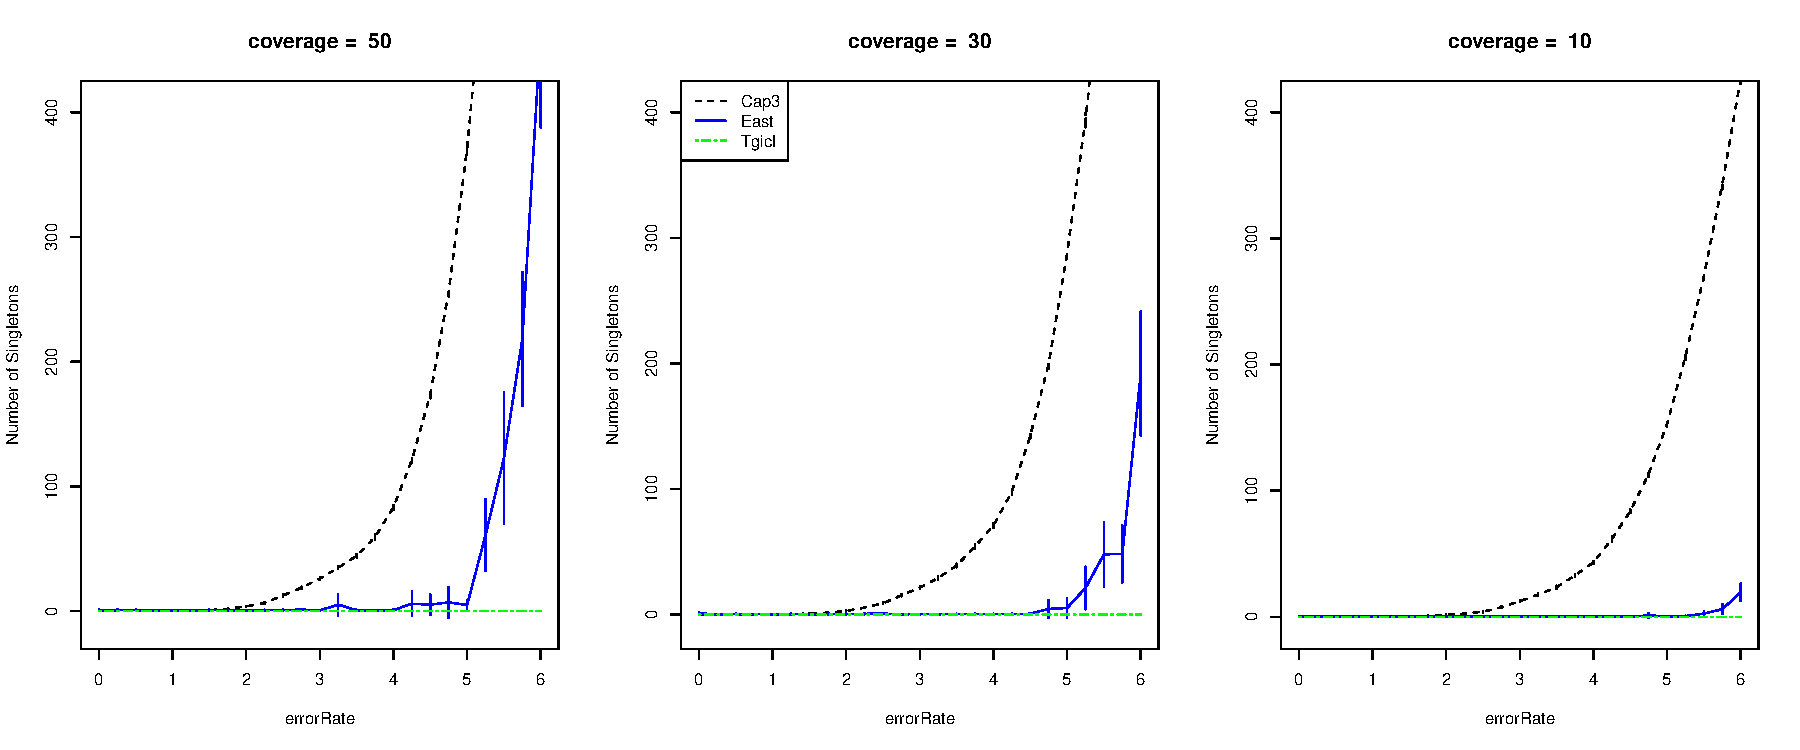
\includegraphics[width=6in]{pics.d/numSingle_sanger.pdf}
\caption{Number of contigs (normalized to the number of transcripts)
  and number of singletons as a function of base-call error
  rate for simulated Sanger sequencing.}
\label{contigsSanger}
\end{figure*}

\noindent {\bf Next Generation Sequences:} In
Figure~\ref{nextgenAscore} we compare the normalized a-score for 454
and Illumina outputs derived from the same zebra fish transcripts
(with sequence lengths averaging 250 and 62 bp respectively).  For
these tests we varied coverage levels but otherwise continued to use
the default Metasim model [\cite{Richter08}].  On 454 data we see
significant improvement in results quality in \east\/ for all levels
of coverage.  On Illumina data we see that \east\/ is competitive with
\velvet\/ at higher coverages, though is unable to match that tool
when coverage is sparse.

\begin{figure*}[htb]
\centerline{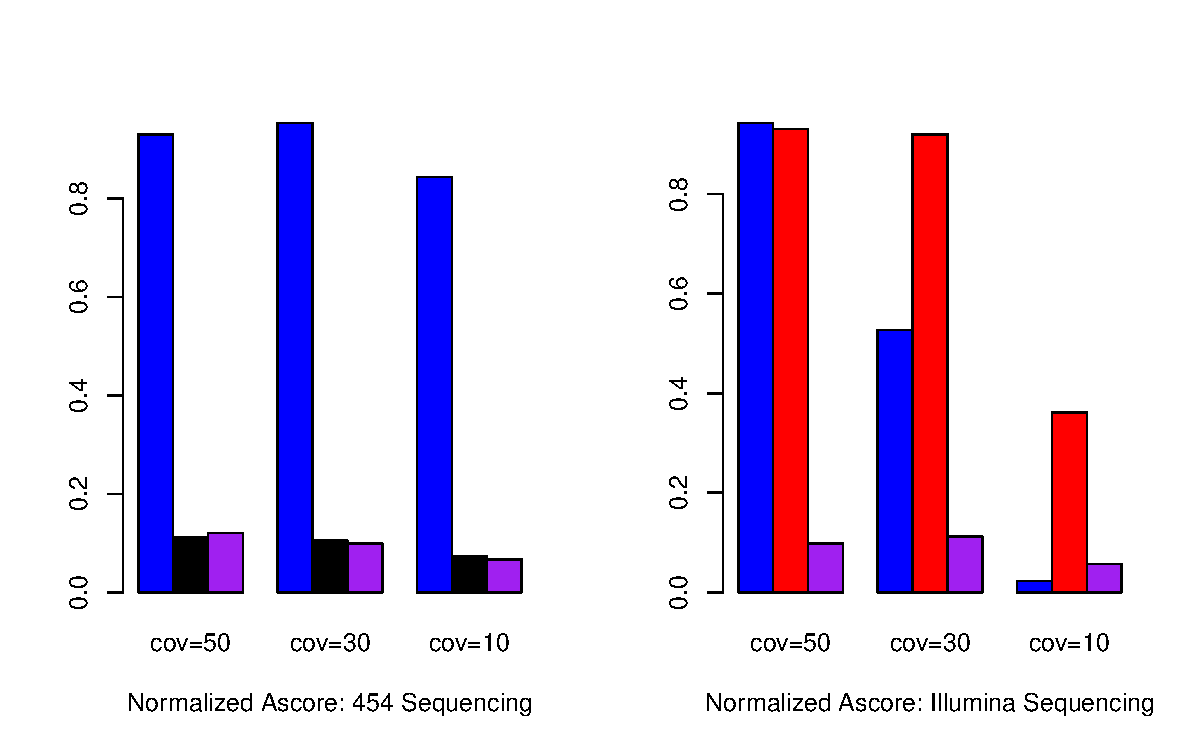
\includegraphics[width=5in]{pics.d/ascore_nxtgen.pdf}}
\caption{Comparative normalized a-scores for 454 and Illumina sequence
  output, using the \metasim default model at different levels
  of coverage.}
\label{nextgenAscore}
\end{figure*}

\noindent {\bf Hybrid:} In Figure~\ref{hybridAscore} we look at the
quality of results derived from applying each tool to a hybrid data
set of Sanger (40\%), 454 (40\%) and Illumina (20\%) sequences, again
showing normalized a-score as a function of base-call error rate in
the Sanger portion.  Here we observe \east\/ matching or outperforming
\capthree\/ and \mira\/ at moderate to high coverages.  At a coverage
level of 50, \east\/ maintains a normalized a-score hovering around
0.85 at all error levels (showing a 54\% improvement over \mira\/ at a
3\% base-call error rate).  \east\/ actually improves its performance
at a coverage level of 30 (hovering around a normalized a-score of
0.95, showing a 142\% improvement over \mira\/ at the 3\% base-call
error rate), an oddity we attribute to the decreased absolute number
of 62bp Illumina sequence.  At a coverage level of 10 \east's
normalized a-score is around 0.37 -- performing considerably worse
than \mira\/ at low error rates (e.g. 0.94 v. 0.40 for error-free
bases), but showing a 52\% improvement over \mira\/ at the 3\% error
rate mark and in general showing increased robustness to error.
Remarkably, it is only in this situation that \capthree\/ is
competitive, with that tool achieving a normalized a-score of 0.62
(v. \east's 0.37) for the 3\% base-call error rate.  However, it does
lose out to \east\/ at greater than a 4.5\% base-call error rate -- a
situation likely due to \east's problems with the 62 bp Illumina
sequences (see below).

\begin{figure*}[htb]
\centerline{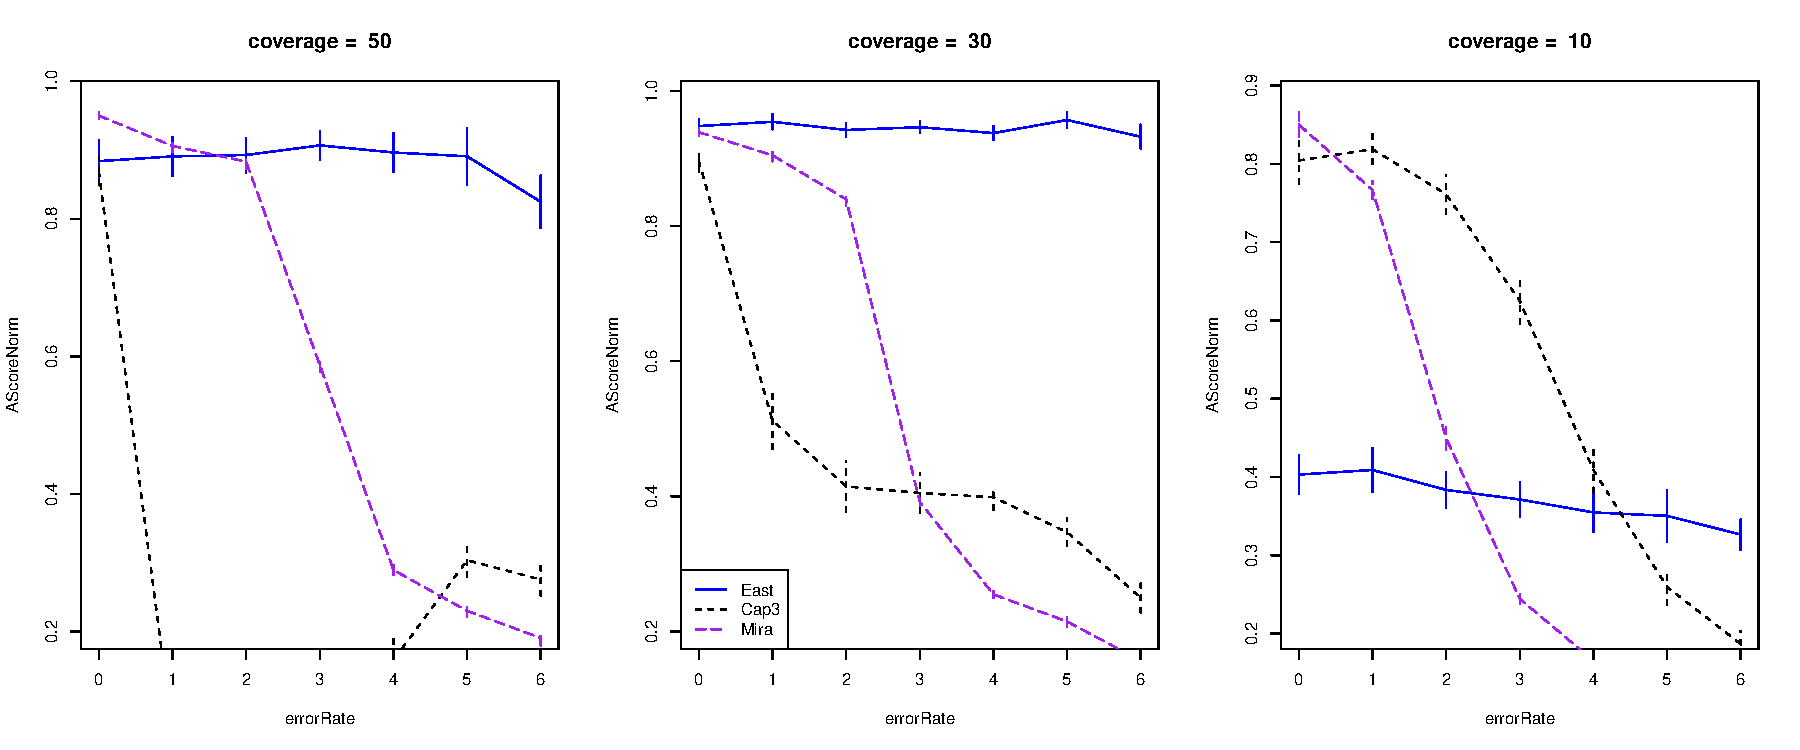
\includegraphics[width=5in]{pics.d/ascore_hybrid.pdf}}
\caption{Comparative normalized a-scores for a hybrid set consisting
  of Sanger, 454 and Illumina sequence output, varying the base-call
  error rate for Sanger sequences and using the MetaSim default model
  for the 454 and Illumina sequences.  Each data set tested was
  composed of 40\% Sanger Sequences, 40\% 454 Sequences, and 20\%
  Illumina sequences.}
\label{hybridAscore}
\end{figure*}

\noindent {\bf Tool Runtime:} In Figures~\ref{runtime.fixed} we see
the average runtime for each of the experiments reflected in
Figures~\ref{sangerAscore}-\ref{hybridAscore} for a coverage of 30
(continuing to report the combined runtime of \peace+\east), while in
Figure~\ref{runtime.coverage} we look at the average runtime for each
tool when applied to simulated data sets generated from a single zebra
fish gene at varying levels of coverage.  For Sanger sequences we
see marked improvement of (\peace+)\east\/ over all other tools for
almost all coverage levels: for the smallest set (coverage = 10)
\east\/ has 1.9 speedup over \capthree\/ and a 3.9 speedup over
\tgicl, while at a more moderate size (coverage=50) there are speedups of
4.7 and 8.4.  This returns back down to 3.0 and 5.2 at the largest set
tested (coverage = 100), as can be seen in the bump around a coverage
of 85 in Figure~\ref{runtime.coverage}.  We are unable to
explain this bump, but have noticed the same effect in
data sets derived from other genes as well.

%\vspace{3mm}

\east\/ is less competitive on shorter sequence.  In our simulations,
we find a reduced runtime improvement on the simulated 454 sequences
(averaging 250 bp in length), and a significantly reduced runtime on
the simulated Illumina sequences (exactly 62 bp in length).  The
increased runtime is due to the problems with applying the $d^2$
metric to short sequences, and will become less of a problem as NGS
technology continues to increase output sequence length
[\cite{Eid09,Li10}]. 


However,
as technology advances, the ``short-read'' sequencers are producing
increasingly longer reads: 454 sequencing technology can produce
reads exceeding 400 bp, while Illumina sequences can exceed 100 bp
[\cite{Eid09,Li10}].  The loss of runtime in our experiments on 454,
Illumina and the hybrid sequences are due to the reduced length
(specifically, the problems with applying the $d^2$ metric to shorter
sequences -- as discussed below), hence are becoming less of an issue
with this increase in short-read fragment length.

%\vspace{3mm}


\begin{figure*}[htb]
\centerline{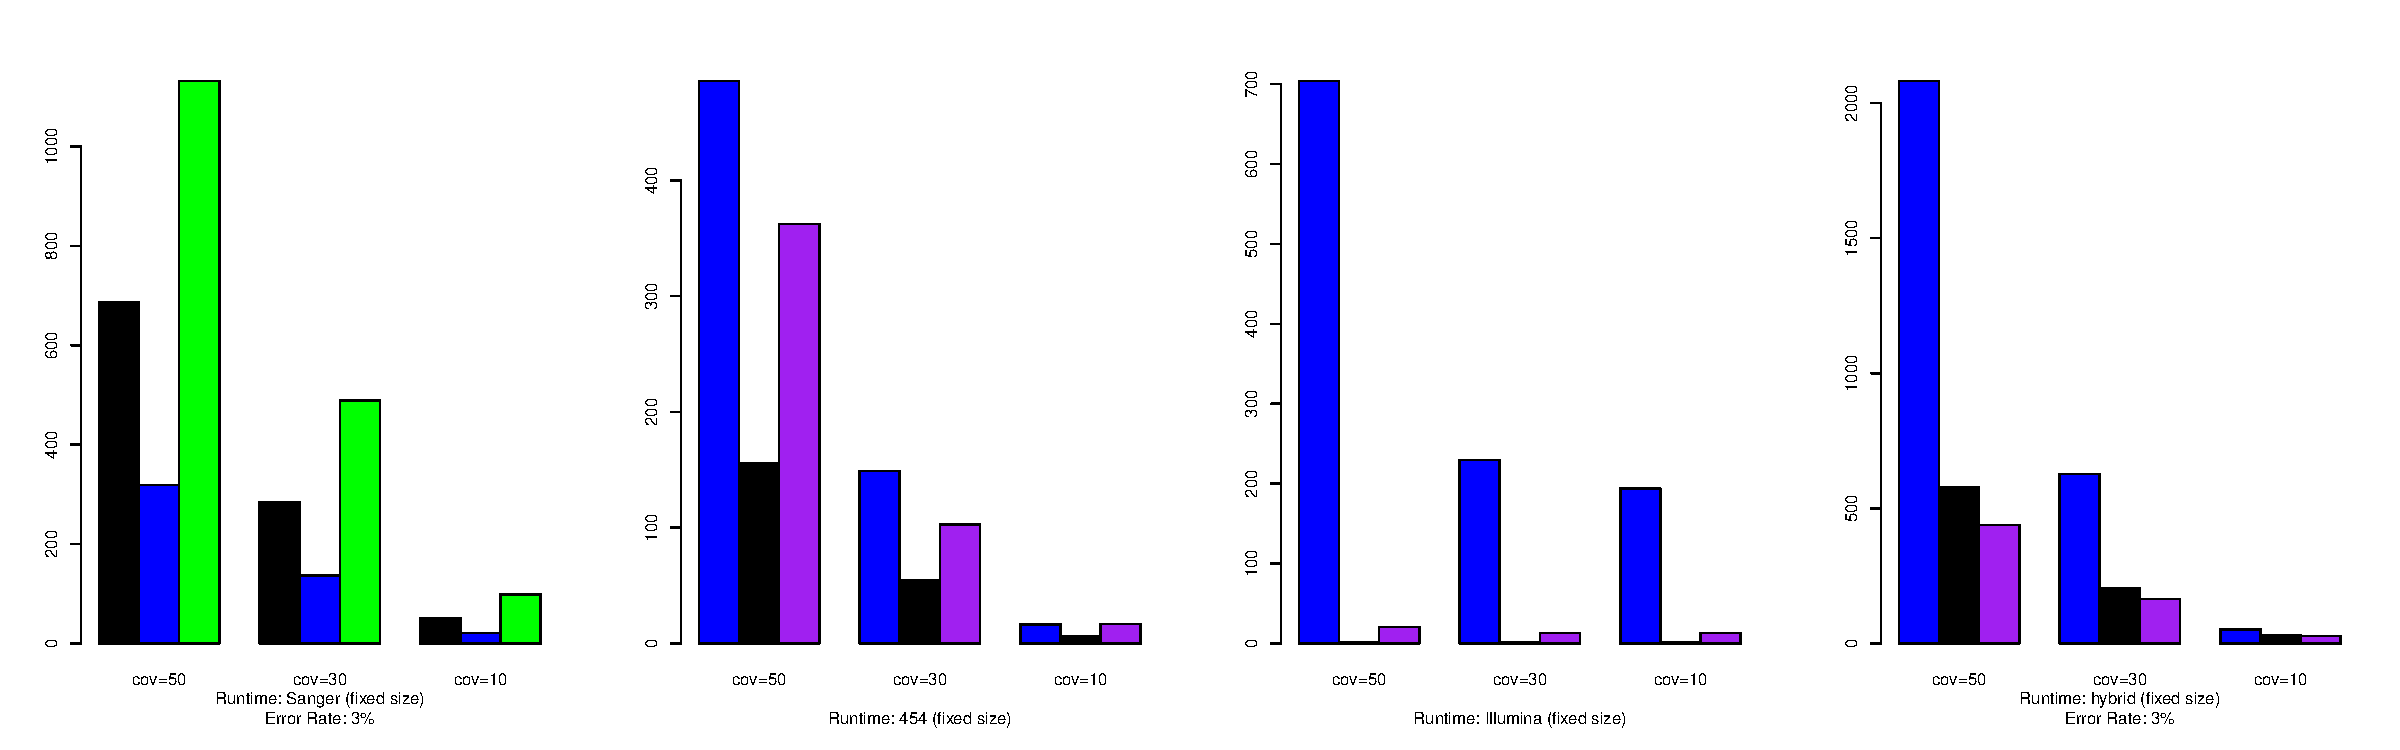
\includegraphics[width=6in]{pics.d/runtime_fixedsize_sanger.pdf}}
\caption{Average runtime per trial when when generating data for
  Figures~\ref{sangerAscore}-\ref{hybridAscore}  when coverage = 30.
  Note that the exceptionally high speed of \velvet\/ on Illumina sequences make the
  red (center) bars in that plot essentially indistinguishable.}
\label{runtime.fixed}
\end{figure*}

\begin{figure*}[htb]
\centerline{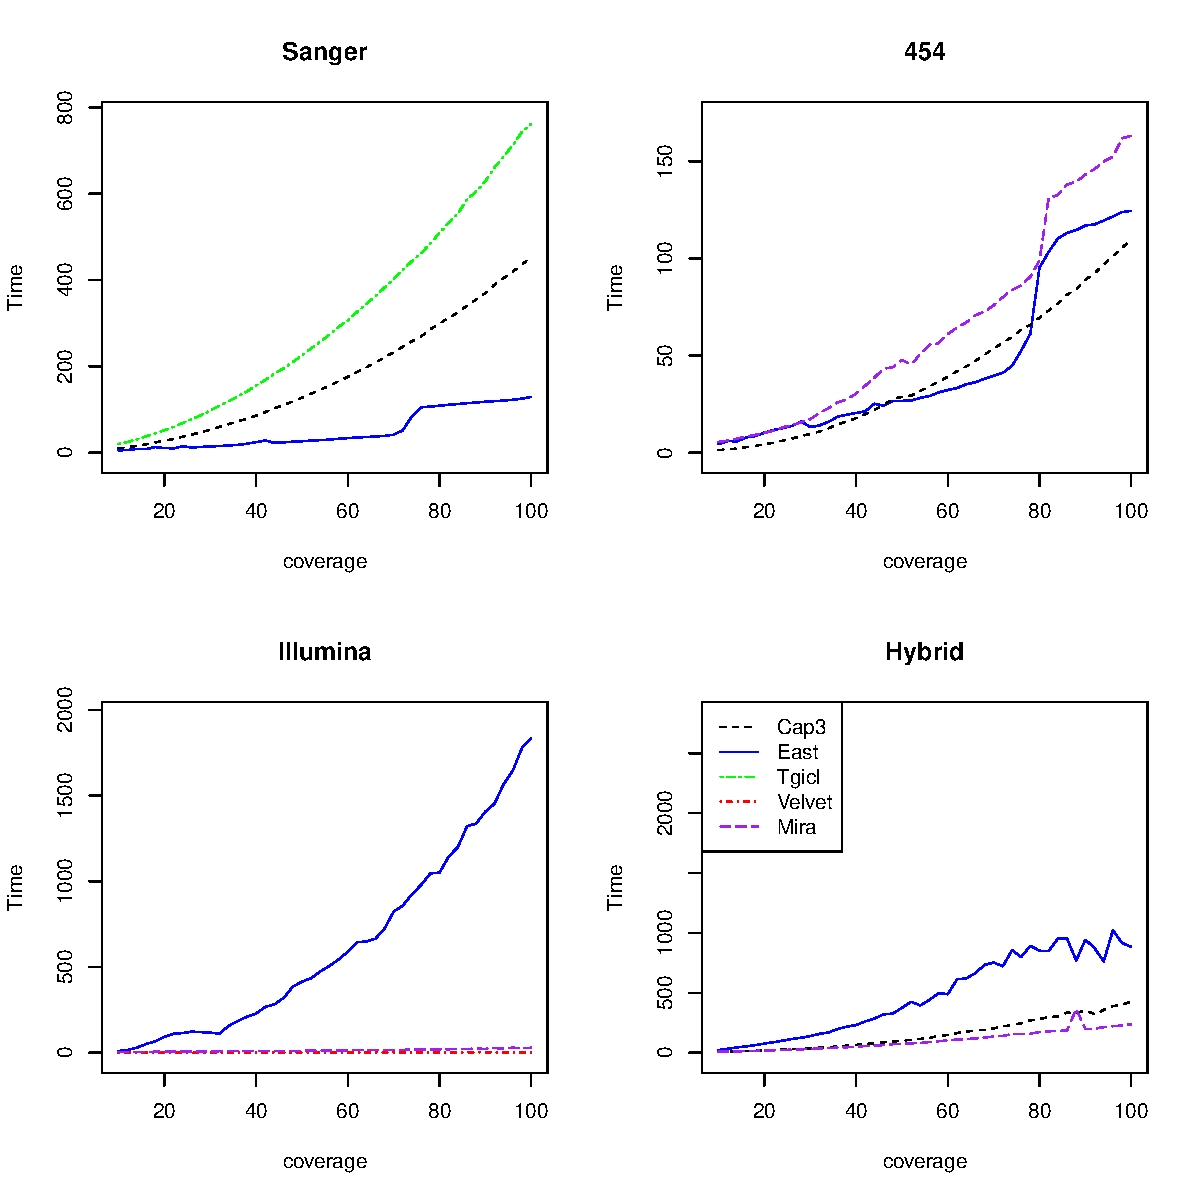
\includegraphics[width=6in]{pics.d/runtime_bycoverage_all.pdf}}
\caption{The average runtime when applying each tool to a simulated
  data set derived from a specific zebrafish transcript of length
  14,625 bp.  As we decrease coverage the number of fragments drops,
  hence illustrating the relationship between tool runtime and
  fragment set size.  Each data point represents the average runtime
  from the application of the tool to at least 30 randomly generated
  simulated sets coming from the transcript at the given level of
  coverage.}
\label{runtime.coverage}
\end{figure*}

%%%%%%%%%%%%%%%%%%%%%%
\section*{Conclusions and Discussion}

\textcolor{blue}{It is said that nothing is perfect, and this statement is certainly
true when discussing assembly tools.  No one assembler can
consistently out performs all other tools, and a user must choose the
the tool that works best for their data.  Our experiments have shown
that the \peast\/ assembly tool produces the best assemblies for Sanger
data with a shorter runtime then competing tools, is the most robust
to sequencing error, and preforms better then any competing tool when
applied to data produced multiple sequencing technology platforms.
\east\/ also demonstrates the viability of the MST-based
approached to sequencing -- an approach we believe has considerable
potential for improvement.}

As observed, when applying \east, \capthree,
and \tgicl\/ to Sanger sequenced transcripts with normal to high error
rates, \east\/ consistently out performs all other tools in terms of
the normalized a-score metric (Figures~\ref{sangerAscore},
\ref{runtime.fixed}, and \ref{runtime.coverage}).  We also find that
the number of contigs produced is almost exactly equal to the number
of transcripts represented in the set, regardless of error rate, while
the number of singleton ESTs remains low up to about a 5\% error rate
(Figures~\ref{contigsSanger}).  The high normalized a-score indicates
that \east\/ is both reconstructing larger portions of each transcript
and doing so more faithfully, while the low number of contigs suggests
that we are assembling complete transcripts.  Finally, runtimes for
\east\/ are considerably faster than other tools for larger sets
(Figures~\ref{runtime.fixed} and \ref{runtime.coverage}), with
(\peace+)\east\/ running a minimum of two to three times as fast as
the other tools.  The speedup over \capthree\/ (the faster tool)
ranged from 1.9 to 6.0, depending on the coverage level.  In short,
when used for Sanger Sequences \east\/ is a faster tool that produces
the high quality reconstructions versus comparing tools and is
significantly more robust to error than other tools.

%\vspace{3mm}

\textcolor{blue}{For Next Generation Sequencing output we see a significant result
quality increase over other tools in many (though not all) situations
(Figures~\ref{nextgenAscore} and \ref{hybridAscore}) -- with \east\/
out performing every tool on 454 data but uncompetitive with \velvet\/
on Illumina data.  This quality does come at a price: the runtime of
\east\/ takes a significant hit when dealing with shorter sequences.
This is due to the dependence of \east\/ on the $d^2$ algorithm, which
has poor performance on shorter sequences.  In practice this does not
pose a large problem: the output sequence length of NGS technology
is continually increasing as the technology advances, leaving
our 62 bp sequence already outdated [\cite{Eid09,Li10}].   These
continuing improvements in runtime, and the improvements in result
quality, justify the \east algorithm as a good choice for assembly.}


Finally, we note, but have not yet explored, the fact that \east\/ is
amenable to to paralilization and the possibility of identifying
isoformes resulting from alternative splicing.  For the first: the
\east\/ tool is trivially parallelizable in that once the \peace\/
portion has completed clustering, \east\/ can address the clusters in
parallel.  More sophisticated paralilization techniques are applicable
at different phased of the east assembly (e.g. the depth-first search
of the MST, or the multiple independent applications of the $d^2$ metric).  


\section*{Acknowledgements}
  Text for this section \ldots

\paragraph{Funding\textcolon} Text Text Text Text Text Text  Text Text.

\bibliography{all}

\end{document}








% LocalWords:  Ozden Chun Liang Karro Botanty publ MSTs et al Hazelhurst Prim's
% LocalWords:  mers Illumina contig bmc multi LaTeX xpression ssembly rees Rao
% LocalWords:  Zhang Moler Dhananjai Mufit de novo introns NGS bruijn ABIITY bp
% LocalWords:  GenBank indels contigs TGICL Metasim MetaSim Runtime runtime pre
% LocalWords:  zebrafish runtimes ESTs paralilization mufit fasta BAM Praveen
% LocalWords:  isophormes XXXXX transcriptome unsequenced transplicing fastaq
% LocalWords:  Kumar
